\subsection{Three prospective interactions predicted from RGB}
\label{sec:rgb-comparison}
Our benchmark asks whether a model fitted to an observed motion episode $D_0$ and optionally updated with one calibrated intervention $D_1$ can predict an independent, held-out action $a_\star$. Ten calibrated cameras provide fitting RGB; camera~0 is reserved for evaluation. Our estimator triangulates RGB tracks from two cameras, uses a known rest geometry, updates a posterior over mechanical hypotheses, and forwards each hypothesis under the test action. Baseline methods fit or adapt their own mechanical representations using the same evidence episodes. The held-out reference remains unavailable until the predictions are sealed. The supplement provides the adapter contracts, provenance and complete case scores.

Three tasks probe complementary predictions. \textbf{S1: Deformable cantilever, changed force direction.} Three cantilevers have equal gravity-driven motion because mass density and elasticity scale proportionally. The test applies a new 20\,N diagonal force at $0.75L$, and we score 3D station displacement over 37 frames. \textbf{S2: Elastic block with hidden stiffness.} A visually homogeneous block conceals an eightfold-stiffer inclusion; a new 30\,N off-centre press is evaluated at 27 surface positions over 25 frames. \textbf{S3: Free striker collision.} The cantilever family is struck by a freely rebounding 0.30\,kg sphere at 1\,m/s; the primary score is absolute axial impulse error, with cantilever displacement as a complementary response metric. There are three reference worlds per task. S1 and S3 share the same three physical objects but test different interactions.

\begin{table*}[t]
\centering
\caption{\textbf{Prediction of new physical interactions after one calibrated observation.} Mean over three synthetic material/inclusion worlds per task (lower is better). All figures use the RGB-only evaluation. The S1, S2, and S3 displacement columns report 3D RMS error in mm; the final column is absolute transferred-impulse error in N\,s.}
\label{tab:benchmark}
\setlength{\tabcolsep}{7pt}
\begin{tabular}{@{}lrrrr@{}}
\toprule
Method & S1: cantilever & S2: block & S3: cantilever & S3: impulse\\
 & RMSE (mm)& RMSE (mm)& RMSE (mm)& Error (N\,s)\\
\midrule
\textbf{Ours (RGB)} & \textbf{1.27} & \textbf{0.33} & \textbf{0.51} & \textbf{0.003}\\
M-PhyGs~\cite{wada2026mphygs} & 5.26 & 1.28 & 3.47 & 0.073\\
PhysTwin~\cite{jiang2025phystwin} & 5.46 & 1.73 & 5.92 & 0.086\\
GIC~\cite{cai2024gic} & 7.21 & 2.60 & 7.97 & 0.069\\
PAC-NeRF~\cite{li2023pacnerf} & 9.45 & 1.78 & 8.27 & 1.771\\
\bottomrule
\end{tabular}
\end{table*}

\begin{figure*}[t]
\centering
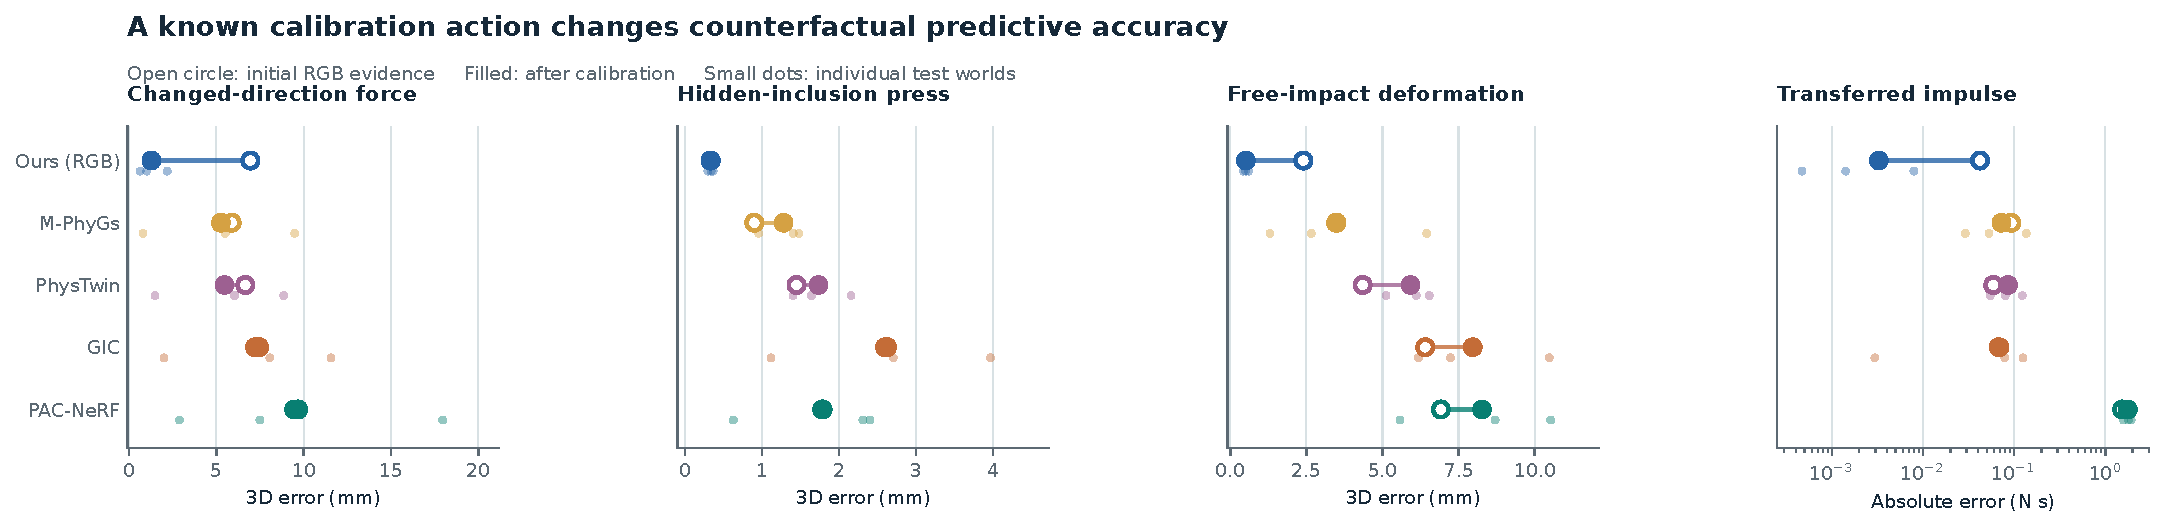
\includegraphics[width=.99\textwidth]{figures/benchmark-deltas.pdf}
\caption{\textbf{Prospective forecasts before and after one calibrated interaction.} Open symbols show mean error using initial RGB evidence; filled symbols show mean after calibration, and smaller dots are individual held-out worlds. Columns measure cantilever force, hidden-inclusion block, free-impact deformation, and transferred impulse. Predictive improvements depend on the action and physical explanation: the block posterior is already concentrated from the first observation.}
\label{fig:benchmark}
\end{figure*}
\begin{figure*}[t]
\centering
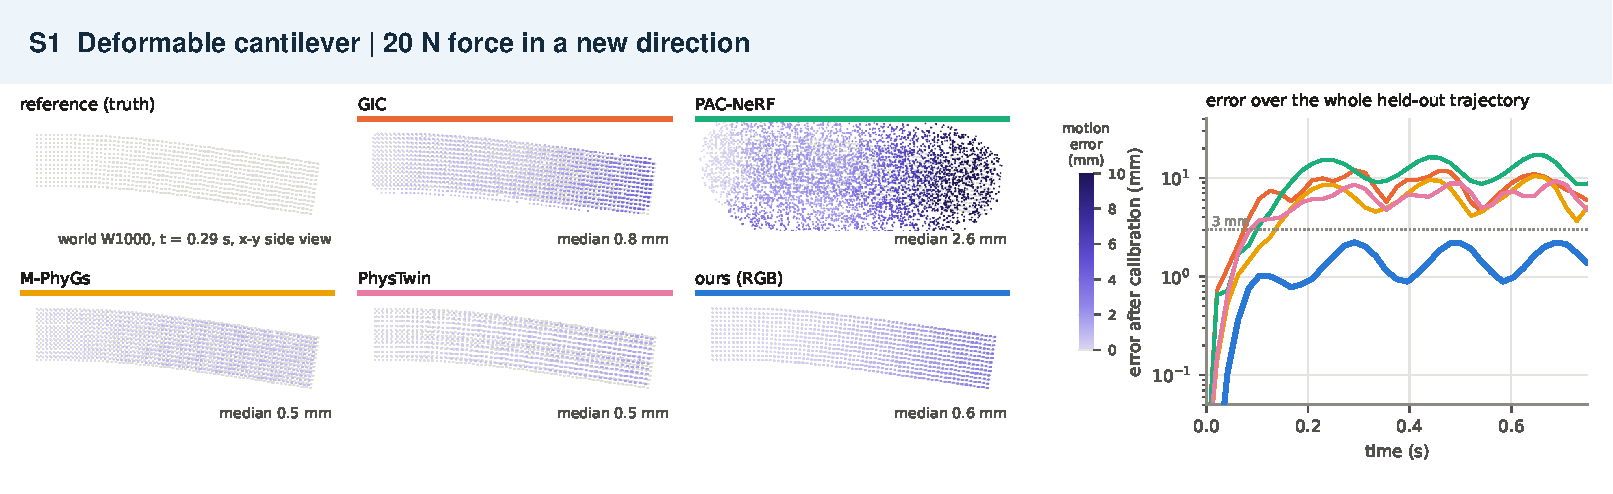
\includegraphics[width=.99\textwidth]{figures/qualitative-S1.pdf}
\caption{\textbf{S1: New-direction cantilever deformation from RGB.} The same reference scene and held-out time are shown for each adapted model after calibration. Surface points are colored by 3D motion error; the right panel plots displacement error over the entire reserved sequence, pooled across the three physical worlds.}
\label{fig:qual-s1}
\end{figure*}
\begin{figure*}[t]
\centering
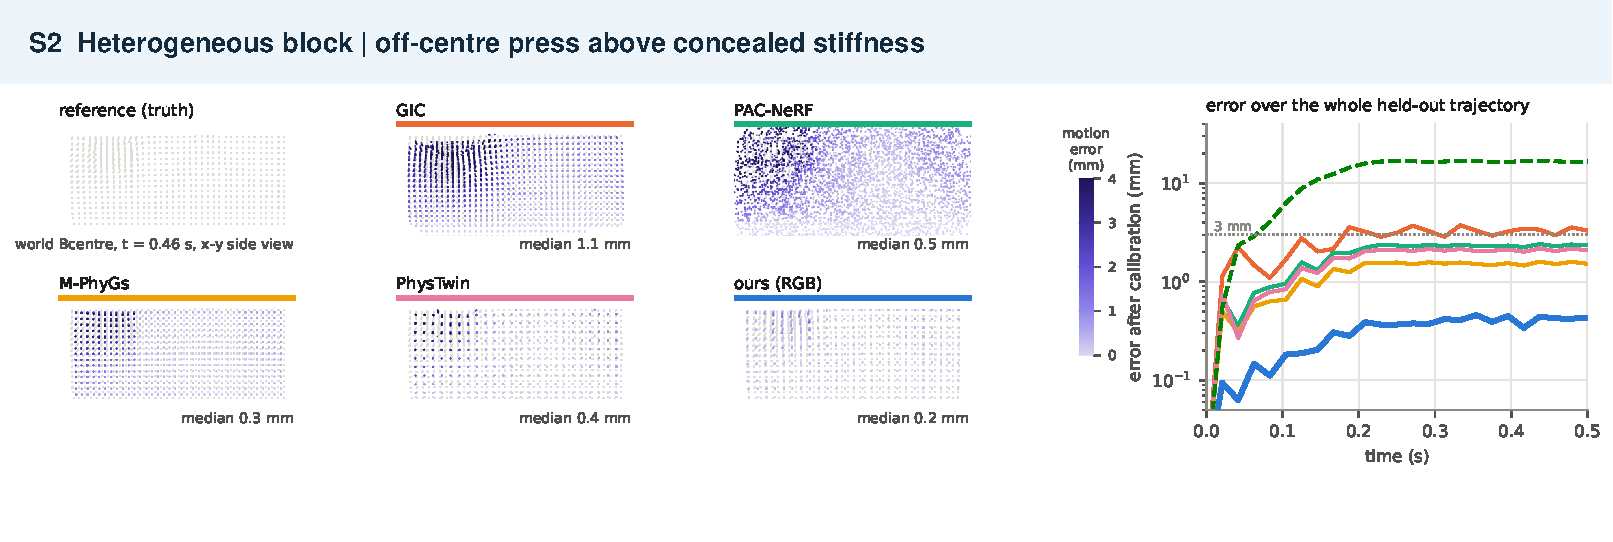
\includegraphics[width=.99\textwidth]{figures/qualitative-S2.pdf}
\caption{\textbf{S2: Novel press over a concealed stiff region.} The predicted physical shape is evaluated against the withheld heterogeneous FEM reference. The last column follows displacement error over the held-out trajectory. The failed spatial-FEM optimization control remains visible as the green dashed curve, with its diagnosis in the supplementary material.}
\label{fig:qual-s2}
\end{figure*}
\begin{figure*}[t]
\centering
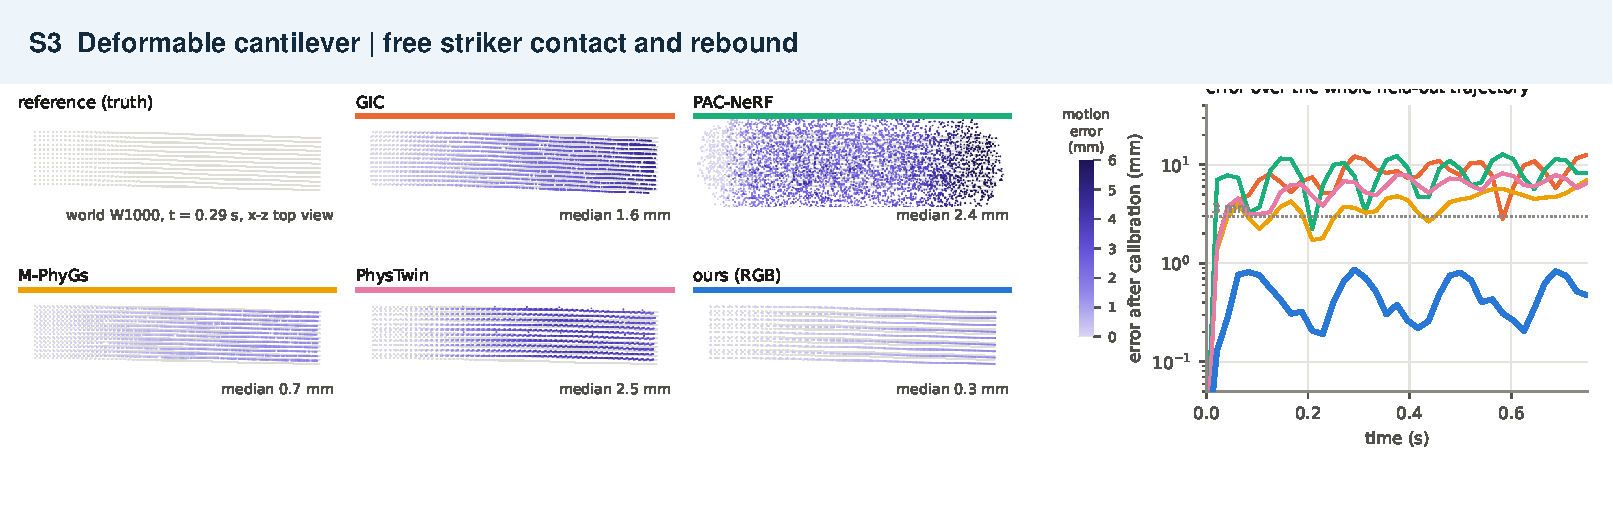
\includegraphics[width=.99\textwidth]{figures/qualitative-S3.pdf}
\caption{\textbf{S3: Deformable cantilever under free striker contact.} All models predict motion after an unseen impact; the figure shows cantilever deformation, while the independent striker-impulse endpoint is reported in Table~\ref{tab:benchmark}. Each method's motion-error trajectory is computed from prospectively sealed predictions.}
\label{fig:qual-s3}
\end{figure*}

\paragraph{Changed-direction cantilever push.}
From $D_0$ alone, our future-action station error is 6.94\,mm, compared with 5.87\,mm for the strongest baseline. The known-force calibration reduces our error to 1.27\,mm (2.18, 1.01 and 0.63\,mm in the three worlds). After the same calibration, M-PhyGs, PhysTwin, GIC and PAC-NeRF score 5.26, 5.46, 7.21 and 9.45\,mm. The target direction differs from both passive gravity and calibration, so the improvement measures transfer to a new force, not re-rendering of the observed action.

\paragraph{Unseen loading of a heterogeneous block.}
Our spatial material-hypothesis bank attains 0.33\,mm mean error, compared with 1.28\,mm for the next comparator. The initial central press already concentrates our finite posterior on one hypothesis; the additional calibration press makes no difference to the resulting prediction. This task therefore probes evidence sufficiency and a spatially resolved physical explanation, rather than an incremental improvement from the second measurement.

\paragraph{Striker momentum and deformation.}
For the free-impact test, calibration reduces our cantilever station error from 2.40 to 0.51\,mm and our absolute striker impulse error from 0.042 to 0.003\,N\,s. The smallest competing post-calibration station error is 3.47\,mm (M-PhyGs), and the smallest competing impulse error is 0.069\,N\,s (GIC). The impulse endpoint tests the mechanical consequences of impact rather than only the visible shape trajectory.

\paragraph{Held-out camera rendering.}
We render all sealed motion forecasts from the reserved camera using one shared GIC-learned Gaussian appearance. This controls the appearance field when measuring the effect of motion. A second, reference-texture visualization transfers the same predictions to the known mesh to increase sensitivity to deformation error. In the shared-appearance test, our post-calibration score is 21.62\,dB on S1 versus 21.64\,dB for reference motion, and 21.75\,dB on S3 versus 21.70\,dB for reference motion. On the block all predictions remain near the shared-appearance 20.72\,dB ceiling even when their displacement errors differ considerably. The reference-texture block rendering instead scores 34.65\,dB for our predicted motion against 28.16\,dB for the best other post-calibration motion. This distinction directly demonstrates that rendering fidelity alone can obscure differences in the underlying physical response.

\subsection{Selecting whether to proceed, look, or probe}
\label{sec:measurement-result}
We independently evaluate evidence acquisition with a compliant-base cantilever model. Ninety-six physical worlds each face three target/visibility settings. Given the initial noisy tip observation, the policy proceeds without measurement in all 96 repeated-load cases (0.104\,mm RMSE). If the target load changes, it requests a view in 92 of 96 cases when base motion is observable (0.073\,mm final RMSE), or a calibrated push in 91 of 96 cases when the base is hidden (0.119\,mm final RMSE). View and probe costs are 0.015 and 0.040 in threshold-failure units at a 0.50\,mm tolerance. The mean decision-loss advantage over a cost-aware Gaussian-moment policy is small, 0.00033, with a bootstrap confidence interval ending at zero. These are fixed-simulator decision experiments; the RGB benchmark above instead applies the same prescribed calibration to every comparator.

\begin{figure*}[t]
\centering
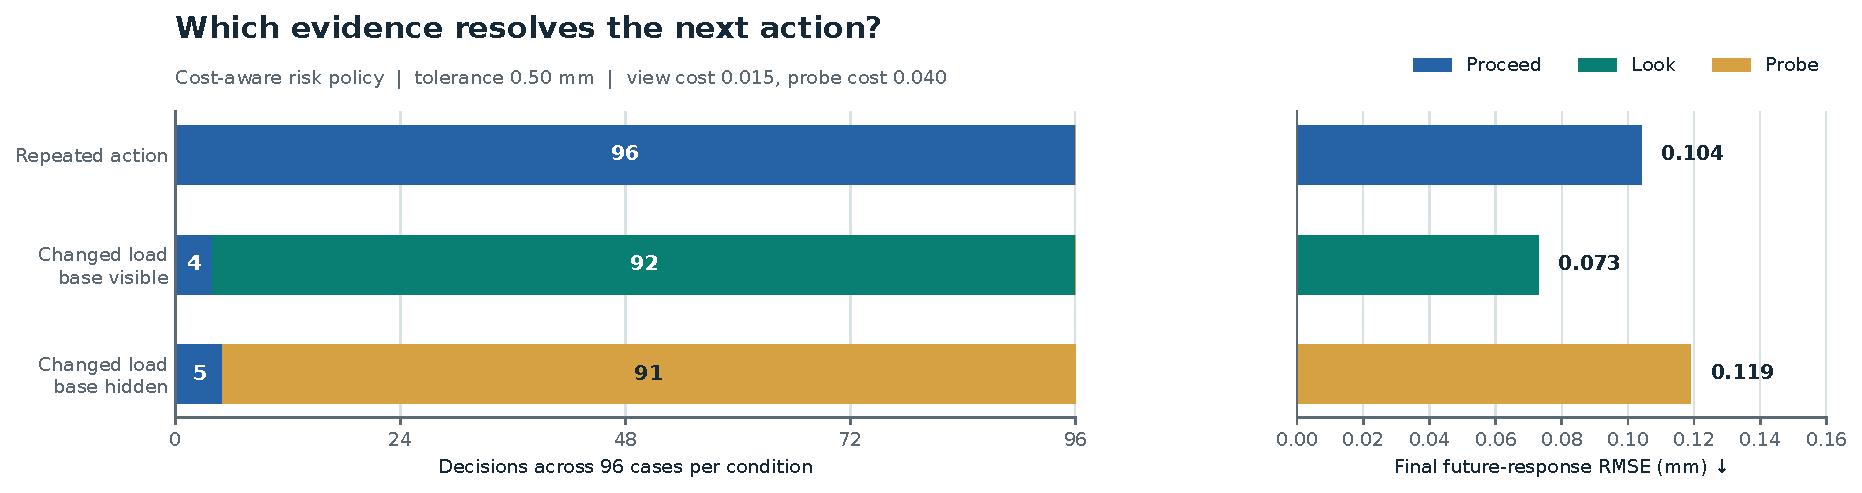
\includegraphics[width=.97\textwidth]{figures/evidence-decision.pdf}
\caption{\textbf{Task-dependent evidence selection.} Over 96 independent cantilever configurations per condition, the posterior risk policy proceeds for the repeated action, generally looks when base motion can be observed, and generally probes when the base is concealed. The adjacent bars show held-out response RMSE after the policy decision. This is a separate controlled decision experiment, not the fixed-calibration RGB benchmark.}
\label{fig:decision}
\end{figure*}

\subsection{Additional independent physical controls}
The original torus continuation experiment separates a time-conditioned appearance forecast from a physics rollout: the GIC deformation network reaches 20.47\,dB on observed motion but 8.29\,dB on future frames, whereas GIC physics and PAC-NeRF achieve 18.44 and 18.01\,dB on that continuation. In a separate three-object drop control, scaling mass, stiffness and damping together yields almost indistinguishable passive movies (94.6--100.1\,dB between simulated movies), but different known-force responses. A contact-model stress experiment estimates 1.86\% risk of exceeding a 3\,mm tolerance while realizing 43.75\% failures when tested against a finer reference. These controls motivate both task-conditioned forecasts and explicit treatment of model mismatch.
